\documentclass{beamer}

\usepackage[utf8]{inputenc}
% \usepackage[french]{babel}
\usepackage{etex}
% \usepackage[hidelinks]{TUL/tulhypref}
% \usepackage[sc]{mathpazo}
\linespread{1.0}
% Si on veut le style de bibliographie named :
%\usepackage{named}

% Pour les figures :
\usepackage{graphicx}

% Si on veut des mini-tables des matières (utiliser minitoc-hyper 
% en conjonction avec tulhypref) :
\usepackage[french]{minitoc}

% \usepackage{titlesec}
\usepackage{url}
\usepackage{listings}
\usepackage{pstricks}
\usepackage{subfigure}
\usepackage{amsmath}
\usepackage{amsthm}
\usepackage{amssymb}
\usepackage{tabularx}
\usepackage{textcomp}
\usepackage{multirow}
\usepackage[algoruled,french,onelanguage]{algorithm2e}
\usepackage[section]{placeins}
\usepackage{xcolor}
\usepackage{colortbl}
\usepackage{longtable}
\usepackage{booktabs}
% \setlength{\aboverulesep}{0pt}
% \setlength{\belowrulesep}{0pt}

\usepackage{epstopdf}
\usepackage{graphicx} % pour insérer des images
\usepackage{stmaryrd}
\usepackage{amsfonts}
% \usepackage{tikz}
% \usepackage{tikz-qtree}
% les figure imbriquées
\usepackage{epsfig}
\usepackage{enumerate}
\usepackage{pifont}
\usepackage{lscape}

\usepackage{pgf}
\usepackage{tikz, calc}
% \usepackage{tikz-cd}
\usetikzlibrary{positioning}
\usetikzlibrary{fit}
\usetikzlibrary{shapes.multipart,calc}
\usetikzlibrary{arrows}

% \usepackage[math]{iwona} 
% \usepackage{iwona} 
% \SetMathAlphabet{\mathtt}{iwona}{OT1}{\ttdefault}{m}{n}

\usepackage[backend=biber, language=french, maxnames=10, citestyle=alphabetic,bibstyle=alphabetic,backref,abbreviate=false,dateabbrev=false,isbn=false,url=false,doi=true]{biblatex}
% \usepackage[backend=biber, language=french, maxnames=5,backref,abbreviate=false,dateabbrev=false,isbn=false,url=false,doi=true]{biblatex}
\addbibresource{these.bib}
% \usepackage[font=small,skip=0pt]{caption}
\usepackage[skip=0pt]{caption}
\usepackage{etoolbox}
\usepackage{needspace}
% \usepackage[zerostyle=a]{newtxtt}

\newcounter{chapter}
% Todo
\newcommand{\done}[1]{\todo[color=green!80!blue!80]{#1}}
\newcommand{\idone}[1]{\todo[inline,color=green!80!blue!80]{#1}}

% Samples
\newcommand{\telock}{tELock}

% Structure
\newtheorem{pb}{Problème}
\newtheorem{theo}{Théorème}
\newtheorem{defi}{Définition}
\newtheorem{prop}{Proposition}
\newtheorem{propri}{Propriété}
\newtheorem{pr}{Preuve}
\newtheorem{cor}{Corollaire}
\newtheorem{rem}{Remarque}
% \theoremstyle{remark}\newtheorem*{preuve}{Preuve}

% % Abbreviations :
\newcommand{\helloworld}{\texttt{Hello World}}
\newcommand{\nasm}{NASM}
\newcommand{\xq}{x86}
\newcommand{\xs}{x86$\_$64}

% Adresses mémoire :
\newcommand{\adr}[1]{$#1$}

% Registres
\newcommand{\eax}{\texttt{eax}}
\newcommand{\ebx}{\texttt{ebx}}
\newcommand{\ecx}{\texttt{ecx}}
\newcommand{\edi}{\texttt{edi}}

% Instructions
\newcommand{\mov}{\texttt{mov}}
\newcommand{\cmp}{\texttt{cmp}}
\newcommand{\add}{\texttt{add}}
\newcommand{\jmp}{\texttt{jmp}}
\newcommand{\ret}{\texttt{ret}}
\newcommand{\call}{\texttt{call}}
\newcommand{\push}{\texttt{push}}
\newcommand{\jne}{\texttt{jne}}
\newcommand{\je}{\texttt{je}}
\newcommand{\sub}{\texttt{sub}}

% Sémantique statique
\newcommand{\BN}{\mathbb N}
\newcommand{\BV}{\mathbb V}
\newcommand{\BX}{\mathbb X}
\newcommand{\BA}{\mathbb A}
\newcommand{\BP}{\mathbb P}
\newcommand{\BT}{\mathbb T}
\newcommand{\BL}{\mathbb L}
\newcommand{\BB}{\mathbb B}
\newcommand{\BNB}{\mathbb N\cup\{\bot\}}
\newcommand{\PN}{\mathcal{P}(\BN)}
\newcommand{\PMN}{\mathcal{P}_M(\BN)}
\newcommand{\Trs}{\mathbb N\cup\{\bot,\top\}}
\newcommand{\TTrs}{\mathcal P(\mathbb V\rightarrow\mathbb N\cup\{\bot,\top\})}
\newcommand{\Tr}{\PN\cup{\top,\bot}}
\newcommand{\TrM}{\PMN\cup\{\top,\bot\}}
\newcommand{\si}{\sigma_{init}}
\newcommand{\specialcell}[2][c]{%
  \begin{tabular}[#1]{@{}l@{}}#2\end{tabular}}
  
% Sémantique dynamique
\newcommand{\CA}{\mathcal A}
\newcommand{\CI}{\mathcal I}
\newcommand{\CC}{\mathcal C}
\newcommand{\CR}{\mathcal R}
\newcommand{\CW}{\mathcal W}
\newcommand{\da}[1]{$\CA[#1]$}
\newcommand{\di}[1]{$\CI[#1]$}
\newcommand{\dc}[1]{$\CC[#1]$}
\newcommand{\dr}[1]{$\CR[#1]$}
\newcommand{\dw}[1]{$\CW[#1]$}

% \usepackage{default}

% \usepackage{graphicx} % pour insérer des images
%\usepackage{graphics} % pour insérer des images vectorielles (ps, eps)
% \usepackage{epstopdf}

% les figure imbriquées
% \usepackage{epsfig}
% \usepackage{subfigure}



% \newtheorem{de}{Définition}
\setbeamertemplate{navigation symbols}{}
% \setbeamercolor{structure}{fg=black!90}
% \setbeamercolor*{palette primary}{use=structure,fg=white,bg=gray!60}
% \setbeamercolor*{palette quaternary}{fg=white,bg=gray!30!black}
% \newtheorem{prop}{Property}

% \usetheme{Warsaw}
 \usetheme{Frankfurt}
%  \setbeamertemplate{mini frames}{}
% \useoutertheme[subsection=false]{miniframes}


\makeatletter
\beamer@compressfalse
\AtBeginDocument{
%     \usebeamerfont*{headline}
    \colorlet{global.bg}{bg}
\pgfdeclareverticalshading{beamer@barshade}{\the\paperwidth}{%
%          color(0ex)=(global.bg);%
         color(0ex)=(section in head/foot.bg);
         color(2ex)=(section in head/foot.bg)% HERE
  }
}
\setbeamertemplate{headline}
{%
  \pgfuseshading{beamer@barshade}%
%   \ifbeamer@sb@subsection%
    \vskip-1.33ex%
%   \else%
%     \vskip-9ex% HERE
%   \fi%
  \begin{beamercolorbox}[ignorebg,ht=0ex,dp=3.75ex]{section in head/foot}
    \insertnavigation{\paperwidth}
% \insertsectionnavigationhorizontal{\paperwidth}{}{\hfill\hfill}
  \end{beamercolorbox}%
%   \ifbeamer@sb@subsection%
%     \begin{beamercolorbox}[ignorebg,ht=2.125ex,dp=1.125ex,%
%       leftskip=.3cm,rightskip=.3cm plus1fil]{subsection in head/foot}
%       \usebeamerfont{subsection in head/foot}\insertsubsectionhead
%     \end{beamercolorbox}%
%   \fi%
  \vskip-3ex% HERE
}%

\makeatother

 \setbeamertemplate{title page}[default][rounded=false]
 \setbeamertemplate{frametitle}[default][colsep=-2bp,rounded=false,shadow=false]
 \setbeamertemplate{blocks}[default]%[rounded=false, shadow=false] 
 \setbeamertemplate{itemize items}[default]
\setbeamertemplate{enumerate items}[default]
%  \setbeamertemplate{frametitle}{\insertframetitle}

% \usecolortheme{wolverine}
%   \usetheme{Berlin}
% \setbeamertemplate{footnote}{%
%   \hangpara{2em}{1}%
%   \makebox[2em][l]{\insertfootnotemark}\footnotesize\insertfootnotetext\par%
% }


\mode<presentation>{
\setbeamertemplate{footline}[frame number] %les numéros de page
\setbeamertemplate{bibliography item}[text]
} 
\title[Désassemblage et détection de logiciels malveillants auto-modifiants]{Désassemblage et détection de logiciels malveillants auto-modifiants}
\author{Aurélien \textsc{Thierry}}% (aurelien@athierry.fr)\\ Équipe CARTE\\ Sous la direction de Jean-Yves Marion}
%\institute{INRIA, Loria}
\date{11 mars 2015}
% \titlegraphic{\includegraphics[width=0.1\textwidth]{../images/loria.jpg}}
% \titlegraphic{\includegraphics[width=0.1\textwidth]{../images/logo_inria.jpg}}


\setbeamersize{text margin left=10pt,text margin right=10pt}

%bleu plus clair
% \setbeamercolor{structure}{fg=blue}

\newcommand{\titre}[1]{
\begin{frame}
  \begin{centering}
    {\usebeamerfont{subsection name}\usebeamercolor[fg]{subsection name}}
    \vskip1em\par
    \begin{beamercolorbox}[sep=8pt,center]{part title}
      \usebeamerfont{subsection title}
      \LARGE #1
      \par
    \end{beamercolorbox}
  \end{centering}
\end{frame}
}

\begin{document}
\makeatletter
  \@ifundefined{inserttotalframenumbernew}{
    \gdef\inserttotalframenumbernew{1}
  }{}
  \gdef\inserttotalframenumber{\inserttotalframenumbernew}
\makeatother

\begin{frame}[plain]
\titlepage
\begin{figure}[ht]
\begin{center}
  \subfigure{
\label{fig:CFGConstr}
\epsfig{figure=TUL/Inria.png,height=1.2cm}}\quad
  \subfigure{
\label{fig:CFGNorm}
\epsfig{figure=TUL/tulloria.pdf,height=1.3cm}}\
\subfigure{
\label{fig:CFGConstr}
\epsfig{figure=TUL/tulul.pdf,height=1.0cm}}\quad
\subfigure{
\label{fig:CFGConstr}
\epsfig{figure=TUL/CNRSfilaire-grand.jpg,height=1.2cm}}\quad
\end{center}
\label{fig:CFGConstrNorm}
% \caption{Virut.a without (99 nodes) and with (41 nodes) reduction}
\end{figure}
\end{frame}

\lstdefinestyle{verbo}{
%     basicstyle=\scriptsize\ttfamily,
    basicstyle=\small\ttfamily,
    breaklines=true,
    breakatwhitespace=true,
    tabsize=1,
    resetmargins=true,
    xleftmargin=0pt,
    frame=none,
    showspaces=false,
    showstringspaces=false
}

\begin{frame}[t]{Introduction}
Objectif : détection de logiciels malveillants (programmes binaires)

\pause
\vskip2ex
Analyse morphologique (Bonfante, Kaczmarek, Marion, 2009) :
\begin{itemize}
 \item Comparaison des graphes de flot de contrôle des programmes
\end{itemize}

\pause
\vskip2ex
Première étape :
\begin{itemize}
 \item Désassemblage d'un programme
 \item Reconstruction d'un graphe de flot de contrôle
\end{itemize}

\pause
\vskip2ex
Obscurcissement :
\begin{itemize}
 \item Chevauchement de code
 \item Auto-modification
\end{itemize}

\pause
\vskip2ex
Seconde étape :
\begin{itemize}
 \item Utilisation de l'analyse morphologique
 \item Formalisation et optimisation de la méthode
 \item Adaptation à la détection de similarités logicielles
\end{itemize}
\end{frame}

\begin{frame}{Binaires et désassemblage}

% \scalebox{1}{
% \begin{tikzpicture}[->,scale=1,>=stealth',thick]
% \node[state] (PC) {Programme C};
% \node[state, right=1.0cm of PC] (ASM) {Programme assembleur};
% \node[state, right=1.0cm of ASM] (BIN) {Fichier binaire};
% 
% % \draw [-] (PC) -- (BIN) {Compilation};
% \draw (PC) -- node[above=0.5cm]{Compilation} (ASM);
% \draw (ASM) -- node[above=0.5cm]{Assemblage} (BIN);
% \end{tikzpicture}}

\begin{center}
\scalebox{1}{
\begin{tikzpicture}[->,scale=1,>=stealth',thick,every text node part/.style={align=center}]
\node[state,draw=none] (PC) {Programme binaire :};
% \node[state, right=1.0cm of PC] (ASM) {\begin{tiny} AB\\BA \end{tiny}};
\node[state, right=0.4cm of PC, text width=1.3cm] (ASM) {\tiny 4d 5a 4b 9c 10 50 00 02 90 21 6d 6e .. .. .. .. 74 50 43 12 00 45 90 00};
\node[state, right=0.1cm of ASM.east, draw=none, anchor = west] (EQ) {=};
\node[state, right=0.8cm of ASM.north east, text width=1.3cm, anchor = north west,minimum size=0.926cm] (HEADER) {Entêtes};
\node[state, below=-0.035cm of HEADER, text width=1.3cm, minimum size=0.926cm] (TEXT) {.text};
\node[state, below=-0.035cm of TEXT, text width=1.3cm, minimum size=0.926cm] (DATA) {.data};

\node[state, right=0.8cm of TEXT.east, anchor = west, draw=none] (PRINTF) {$\sim$\ printf()};
\node[state, right=0.8cm of DATA.east, anchor = west, draw=none] (HELLO) {``Hello, World''};
% \node[state, right=1.0cm of ASM] (BIN) {Fichier binaire};
% \draw [-] (PC) -- (BIN) {Compilation};
% \draw (PC) -- node[left=0.7cm]{Assemblage} (ASM);
\draw [-] (TEXT) -- (PRINTF);
\draw [-] (DATA) -- (HELLO);
% \draw (ASM) -- node[above=0.5cm]{Assemblage} (BIN);
\end{tikzpicture}}
\end{center}

\pause
% \begin{tabular}[b]{|l|}
% \hline
% Entêtes\\
% \hline
% Sections\\
% ~~~~.text\\
% \hline
% ~~~~.data\\
% \hline
% ~~~~...\\
% \hline
% \end{tabular}
Désassemblage :
\begin{itemize}
 \item Programme binaire $\rightarrow$ code assembleur
 \item Code et données peuvent être présents dans les mêmes sections
 \item Difficile de séparer les données du code
\end{itemize}

\pause
\begin{defi}
 Le désassemblage parfait d'un programme binaire est la donnée de l'ensemble de ses instructions atteignables.
\end{defi}
Il s'agit d'un problème indécidable.
\end{frame}

% \begin{frame}{Désassemblage et graphe de flot de contrôle}
% % \begin{center}
% % \only<1>{
% % \begin{table}
% % % \small
% % \begin{tabular}[b]{|l|l|l|}
% % \hline
% % Adresse & Octets & Instruction\\ 
% % \hline
% %  8048067  &  b8 00 00 00 00         &  mov    eax,0x0 \\
% %  804806c  &  eb 05                  &  jmp    0x8048073 \\
% %  804806e  &  b8 03 00 00 00         &  mov    eax,0x3 \\
% %  8048073  &  83 f8 00               &  cmp    eax,0x0 \\
% %  8048076  &  74 06                  &  je     0x804807e \\
% %  8048078  &  b8 01 00 00 00         &  mov    eax,0x1 \\
% %  804807d  &  c3                     &  ret     \\
% %  804807e  &  b8 02 00 00 00         &  mov    eax,0x2 \\
% %  8048083  &  c3                     &  ret     \\
% % \hline
% % \end{tabular}
% % \end{table}
% % }
% \begin{minipage}{.5\textwidth}
%   \centering
%   \footnotesize
%   \begin{table}
% % \small
% \begin{tabular}[b]{|l|l|l|}
% \hline
% Adresse & Octets & Instruction\\ 
% \hline
%  8048067  &  b8 00 00 00 00         &  mov    eax,0x0 \\
%  804806c  &  eb 05                  &  jmp    0x8048073 \\
%  804806e  &  b8 03 00 00 00         &  mov    eax,0x3 \\
%  8048073  &  83 f8 00               &  cmp    eax,0x0 \\
%  8048076  &  74 06                  &  je     0x804807e \\
%  8048078  &  b8 01 00 00 00         &  mov    eax,0x1 \\
%  804807d  &  c3                     &  ret     \\
%  804807e  &  b8 02 00 00 00         &  mov    eax,0x2 \\
%  8048083  &  c3                     &  ret     \\
% \hline
% \end{tabular}
% \end{table}
% \end{minipage}%
% \begin{minipage}{.6\textwidth}
%   \centering
%   \includegraphics[width=0.65\textwidth]{supports/eax-cfg/eax2_cropped0.pdf}
% \end{minipage}
% 
% % \pause
% % % \vskip-3ex
% % Difficultés :
% % \begin{itemize}
% %  \item Chevauchement de code : instructions codées sur les mêmes adresses
% %  \item Auto-modification : code non constant au courant de l'exécution
% % \end{itemize}
% % \end{center}
% \end{frame}



% \begin{frame}{Plan et \underline{contributions}}
% Analyse de programmes binaires obscurcis
% \begin{itemize}
%  \item Désassemblage et obscurcissement
%  \item \underline{Analyse statique du chevauchement de code}
%  \item Analyse dynamique de l'auto-modification
%  \item \underline{Graphe de flot de contrôle pour programmes auto-modifiants}
% %  \item \underline{Présentation d'un désassembleur hybride}
% \end{itemize}
% 
% \vspace{1cm}
% Détection de programmes malveillants
% \begin{itemize}
%  \item Comparaison des graphes de flot de contrôle
%  \item \underline{Formalisation et optimisation}
%  \item \underline{Exemples d'application}
% \end{itemize}
% 
% \end{frame}

\section{Analyse statique}
% \subsection{Difficultés}

\begin{frame}[t]{Désassemblage et graphe de flot de contrôle}
\begin{minipage}{.5\textwidth}
  \centering
  \footnotesize
  \begin{table}
% \small
\begin{tabular}[b]{|l|l|l|}
\hline
Adresse & Octets & Instruction\\ 
\hline
 8048067  &  b8 00 00 00 00         &  mov    eax,0x0 \\
 804806c  &  eb 05                  &  jmp    0x8048073 \\
 804806e  &  b8 03 00 00 00         &  mov    eax,0x3 \\
 8048073  &  83 f8 00               &  cmp    eax,0x0 \\
 8048076  &  74 06                  &  je     0x804807e \\
 8048078  &  b8 01 00 00 00         &  mov    eax,0x1 \\
 804807d  &  c3                     &  ret     \\
 804807e  &  b8 02 00 00 00         &  mov    eax,0x2 \\
 8048083  &  c3                     &  ret     \\
\hline
\end{tabular}
\end{table}
\end{minipage}%
\begin{minipage}{.6\textwidth}
  \centering
  \includegraphics[width=0.65\textwidth]{supports/eax-cfg/eax2_cropped0.pdf}
\end{minipage}

% \pause
\vskip-0.5ex
\only<2>{
Désassemblage linéaire :
\begin{itemize}
%  \item Parcourt la première instruction du binaire puis l'instruction à l'adresse suivante
 \item Désassemblage adresse après adresse
\end{itemize}

Désassemblage récursif :
\begin{itemize}
 \item Suit le flot de contrôle des instructions
 \item Jusqu'à un retour (\ret) ou un saut dynamique (\texttt{jmp eax})
%  \item Parcourt le point d'entrée puis les instructions pouvant potentiellement la suivre à l'exécution
%  \item Donne une approximation des instructions potentiellement exécutées
%  \item Problème des sauts dynamiques : \texttt{jmp eax}
\end{itemize}
}

\only<3>{
% \frametitle{Désassemblage récursif : graphe de flot de contrôle (GFC)}
% Graphe de flot de contrôle (GFC) :
% \begin{itemize}
%  \item Donne une sur-approximation des instructions potentiellement exécutées
% \end{itemize}
% \begin{defi}
 Graphe de flot de contrôle parfait (théorique) :
 \begin{itemize}
  \item On suppose qu'on dispose de toutes les exécutions possibles
  \item Sommets : ensemble des couples (adresse, instruction) atteignables
  \item Arc entre $a$ et $b$ ssi il existe un chemin d'exécution au sein duquel $b$ suit immédiatement $a$
 \end{itemize}
\label{def:cfg_parfait_nsm}
% \end{defi}
}

\only<4>{
\vskip5ex
Objectif : désassemblage et reconstruction automatique du GFC
}
\end{frame}

\begin{frame}{Obscurcissement}
But de l'attaquant : rendre le désassemblage plus difficile
\begin{itemize}
 \item Compression, chiffrement, ajout de code inutile...
 \pause
 \item En pratique appliqué par un logiciel d'empaquetage
\end{itemize}

\begin{center}
\scalebox{0.8}{
\begin{tikzpicture}[->,scale=1,>=stealth',thick]
\node[state, text width=3cm, minimum size=2cm] (BIN){Binaire d'origine};
\node[state, below right = -0.5cm and 4cm of BIN.east, text width=3cm, minimum size=2cm] (BINO){Données :\\Binaire d'origine caché};
\node[state, below = -2cm of BINO.north, text width=3cm, minimum size=2cm] (UNPACK){Code :\\Routine de dépaquetage};
% \draw ($(BIN.north west) + (-0.8, -0.1) $) -- node[left=0.3cm]{Point d'entrée} ($(BIN.north west) + (0, -0.1) $);
% \draw ($(UNPACK.north east) + (0.8, -0.1) $) -- node[right=0.3cm]{Point d'entrée} ($(UNPACK.north east) + (0, -0.1) $);
\draw ($(BIN.east) + (0.5, 0) $) -- node[below]{\large Enpaquetage} ($(BIN.east) + (3cm, 0) $);
\node [fit={($(UNPACK.north west) + (-0.1, 0.1)$) ($(BINO.south east) + (0.1, -0.1)$)}, draw, label=Binaire empaqueté] {};
\end{tikzpicture}
}
\end{center}

\telock\ :
\begin{itemize}
 \item Chevauchement de code, auto-modification
\end{itemize}

\end{frame}

% \begin{frame}{Désassemblage récursif et graphe de flot de contrôle}
% \begin{minipage}{.5\textwidth}
%   \centering
%   \begin{table}
% %   \tiny
%   \begin{tabular}[b]{|l|}
%   \hline
%   Instructions\\ 
%   \hline
%   mov    eax,0x0 \\
%   jmp    0x8048073 \\
%   mov    eax,0x3 \\
%   cmp    eax,0x0 \\
%   je     0x804807e \\
%   mov    eax,0x1 \\
%   ret     \\
%   mov    eax,0x2 \\
%   ret     \\
%   \hline
%   \end{tabular}
%   \end{table}
% \end{minipage}%
% \begin{minipage}{.45\textwidth}
%   \centering
%   \includegraphics[width=0.8\textwidth]{supports/eax-cfg/eax2_cropped0.pdf}
% \end{minipage}
% 
% 
% \end{frame}


\titre{Chevauchement de code et analyse statique}
\begin{frame}[t,fragile]{Chevauchement de code}
\vskip-2.5ex
\begin{itemize}
%  \item Technique d'obscurcissement statique
 \item Plusieurs instructions codées sur des adresses qui se chevauchent
 \item Assembleur \xq\ : taille des instructions variable (entre 1 et 15 octets)
 \item Les désassembleurs (IDA) font généralement l'hypothèse que ce n'est pas le cas
\end{itemize}

% \vskip-2ex
\begin{block}{Exemple (\telock)}
Octets à désassembler : \texttt{eb ff c9 7f e6}
\begin{lstlisting}[language={[x86masm]Assembler}, escapechar=~]
01006e7d    eb ff           jmp +1
01006e7e       ff c9        dec ecx
01006e80    7f e6           jg 01006e68
\end{lstlisting}
\pause
\end{block}

% \vskip-2ex
\begin{itemize}
 \item Possibilité de cacher une séquence de code de longueur arbitraire au milieu d'un autre code\only<2>{\footnote{Jämthagen, Lantz et Hell (2013)}}
\end{itemize}


\end{frame}

\begin{frame}[fragile]{Chevauchement de code : sémantique}
\begin{block}{Exemple (\telock)}
Octets à désassembler : \texttt{eb ff c9 7f e6}
\begin{lstlisting}[language={[x86masm]Assembler}, escapechar=~]
01006e7d    eb ff           jmp +1
01006e7e       ff c9        dec ecx
01006e80    7f e6           jg 01006e68
\end{lstlisting}
\end{block}

\begin{itemize}
 \item Séparation des instructions en couches de code
\end{itemize}


\begin{center}
\begin{table}
\small
\begin{tabular}{|l|c|c|c|c|c|}
\hline
Adresses & 01006e7d & 01006e7e & 01006e7f & 01006e80 & 01006e81\\
\hline
Octets & eb & ff & c9 & 7f & e6\\
\hline
\Layer\ 1 & \multicolumn{2}{c|}{jmp +1} & leave & \multicolumn{2}{c|}{jg 0x1006e68}\\
\hline
\Layer\ 2 & \cnoir & \multicolumn{2}{c|}{dec ecx} & \multicolumn{2}{c|}{\cnoir} \\
 \hline
% \\
\end{tabular}
\end{table}
\end{center}
\end{frame}



\begin{frame}[fragile]{Chevauchement de code : sémantique}
% \only<1-2>{
% \begin{table}
% \small
% \begin{tabular}{|l|c|c|c|c|c|}
% \hline
% Adresses & 01006e7d & 01006e7e & 01006e7f & 01006e80 & 01006e81\\
% \hline
% Octets & eb & ff & c9 & 7f & e6\\
% \hline
% \Layer\ 1 & \multicolumn{2}{c|}{jmp +1} & \cnoir & \multicolumn{2}{c|}{jg 0x1006e68}\\
% \hline
% \Layer\ 2 & \cnoir & \multicolumn{2}{c|}{dec ecx} & \multicolumn{2}{c|}{\cnoir} \\
%  \hline
% % \\
% \end{tabular}
% \end{table}

Couche de code :
\begin{itemize}
 \item Ensemble d'instructions qui ne se chevauchent pas.
\end{itemize}

\begin{defi}
 Étant donné un ensemble d'instructions $E$, un découpage cohérent est un ensemble de \layers\
 \begin{itemize}
  \item deux à deux disjointes,
  \item recouvrant l'ensemble des instructions $E$.
 \end{itemize}
\label{def:decoupage}
\end{defi}
% }

\pause
% \only<2>{
Quelle stratégie pour construire un découpage cohérent en couches ?
\begin{itemize}
 \item Couches linéaires
 \item Couches désassemblées par parcours récursif
\end{itemize}

% }
\end{frame}

\begin{frame}[t]{Chevauchement de code : couches linéraires}
% Couches linéaires :
\begin{itemize}
 \item Une couche démarre à chaque adresse et consiste en un désassemblage linéaire
 \item Les couches inférieures redondantes sont supprimées
\end{itemize}
\only<1>{
\begin{center}
\begin{tabular}{|l|c|c|c|c|c|}
\hline
Adresses & 01006e7d & 01006e7e & 01006e7f & 01006e80 & 01006e81\\
\hline
Octets & eb & ff & c9 & 7f & e6\\
\hline
\Layer\ 1 & \multicolumn{2}{c|}{jmp +1} & leave & \multicolumn{2}{|c|}{jg 0x1006e68}\\
\hline
\Layer\ 2 & \cnoir & \multicolumn{2}{c|}{dec ecx} & \multicolumn{2}{|c|}{jg 0x1006e68 \cgris} \\
\hline
\Layer\ 3 & \multicolumn{2}{c|}{\cnoir} & leave \cgris & \multicolumn{2}{|c|}{jg 0x1006e68 \cgris} \\
\hline
\Layer\ 4 & \multicolumn{3}{c|}{\cnoir} & \multicolumn{2}{|c|}{jg 0x1006e68 \cgris} \\
\hline
\Layer\ 5 & \multicolumn{4}{|c|}{\cnoir} & (invalide) \\
\hline
% \\
\end{tabular}
\end{center}
}
\only<2->{
\begin{center}
\begin{tabular}{|l|c|c|c|c|c|}
\hline
Adresses & 01006e7d & 01006e7e & 01006e7f & 01006e80 & 01006e81\\
\hline
Octets & eb & ff & c9 & 7f & e6\\
\hline
\Layer\ 1 & \multicolumn{2}{c|}{jmp +1} & leave & \multicolumn{2}{|c|}{jg 0x1006e68}\\
\hline
\Layer\ 2 & \cnoir & \multicolumn{2}{c|}{dec ecx} & \multicolumn{2}{|c|}{jg 0x1006e68 \cgris} \\
\hline
% \\
\end{tabular}
\end{center}
}

\pause
\pause
\begin{itemize}
 \item La première couche correspond au désassemblage linéaire
 \item L'ensemble des couches est une généralisation du désassemblage linéaire
\end{itemize}
\end{frame}

\begin{frame}{Couches désassemblées par parcours récursif}
% Couches linéaires :
\begin{itemize}
 \item On suit le parcours réalisé lors du désassemblage
 \item On ajoute chaque instruction désassemblée à la première couche existante pouvant la contenir, ou à une nouvelle couche
\end{itemize}

% \pause
\begin{center}
\begin{tabular}{|l|c|c|c|c|c|}
\hline
Adresses & 01006e7d & 01006e7e & 01006e7f & 01006e80 & 01006e81\\
\hline
Octets & eb & ff & c9 & 7f & e6\\
\hline
\Layer\ 1 & \multicolumn{2}{c|}{jmp +1} & \cnoir & \multicolumn{2}{c|}{jg 0x1006e68}\\
\hline
\Layer\ 2 & \cnoir & \multicolumn{2}{c|}{dec ecx} & \multicolumn{2}{c|}{\cnoir} \\
 \hline
% \\
\end{tabular}
\end{center}

% \pause
\begin{itemize}
 \item Permet d'observer les difficultés liées au chevauchement de code lors du désassemblage récursif
\end{itemize}


\end{frame}

\begin{frame}[t]{Chevauchement de code : Caractérisation}
\begin{center}
\begin{tabular}{|l|c|c|c|c|c|}
\hline
Adresses & 01006e7d & 01006e7e & 01006e7f & 01006e80 & 01006e81\\
\hline
Octets & eb & ff & c9 & 7f & e6\\
\hline
\Layer\ 1 & \multicolumn{2}{c|}{jmp +1} & \cnoir & \multicolumn{2}{c|}{jg 0x1006e68}\\
\hline
\Layer\ 2 & \cnoir & \multicolumn{2}{c|}{dec ecx} & \multicolumn{2}{c|}{\cnoir} \\
 \hline
% \\
\end{tabular}
\end{center}

\only<1>{
Métriques :
\begin{itemize}
 \item Binaire non obscurci : désassemblage récursif constitué d'une seul couche
 \item Nombre de couches : indique la complexité des chevauchements
 \item Nombre de sauts de changement de couches : indique la fréquence d'utilisation de cette technique
\end{itemize}
}

% \only<2>{
%  \begin{center}
% \includegraphics[width=0.7\textwidth]{supports/disasm/telock/telock_cropped0.pdf}
% \end{center}
% }
\end{frame}
% 
% \begin{frame}{Chevauchement de code : graphe de flot de contrôle}
% % \begin{minipage}{.5\textwidth}
% \begin{center}
% \begin{tabular}{|l|c|c|c|c|c|}
% \hline
% Adresses & 01006e7d & 01006e7e & 01006e7f & 01006e80 & 01006e81\\
% \hline
% Octets & eb & ff & c9 & 7f & e6\\
% \hline
% \Layer\ 1 & \multicolumn{2}{c|}{jmp +1} & \cnoir & \multicolumn{2}{c|}{jg 0x1006e68}\\
% \hline
% \Layer\ 2 & \cnoir & \multicolumn{2}{c|}{dec ecx} & \multicolumn{2}{c|}{\cnoir} \\
%  \hline
% % \\
% \end{tabular}
% \end{center}
% % \end{minipage}
% 
% 
% % \begin{minipage}{.5\textwidth}
% 
% % \end{minipage}
% \end{frame}


\section{Analyse dynamique}
\titre{Auto-modification et analyse dynamique}

\begin{frame}{Auto-modification}
Problème : certains programmes se modifient pendant l'exécution
\begin{itemize}
 \item Découpage en niveaux d'exécution (Reynaud, Calvet)
 \item Utilisation d'une analyse dynamique (trace d'exécution)
\end{itemize}

\begin{center}
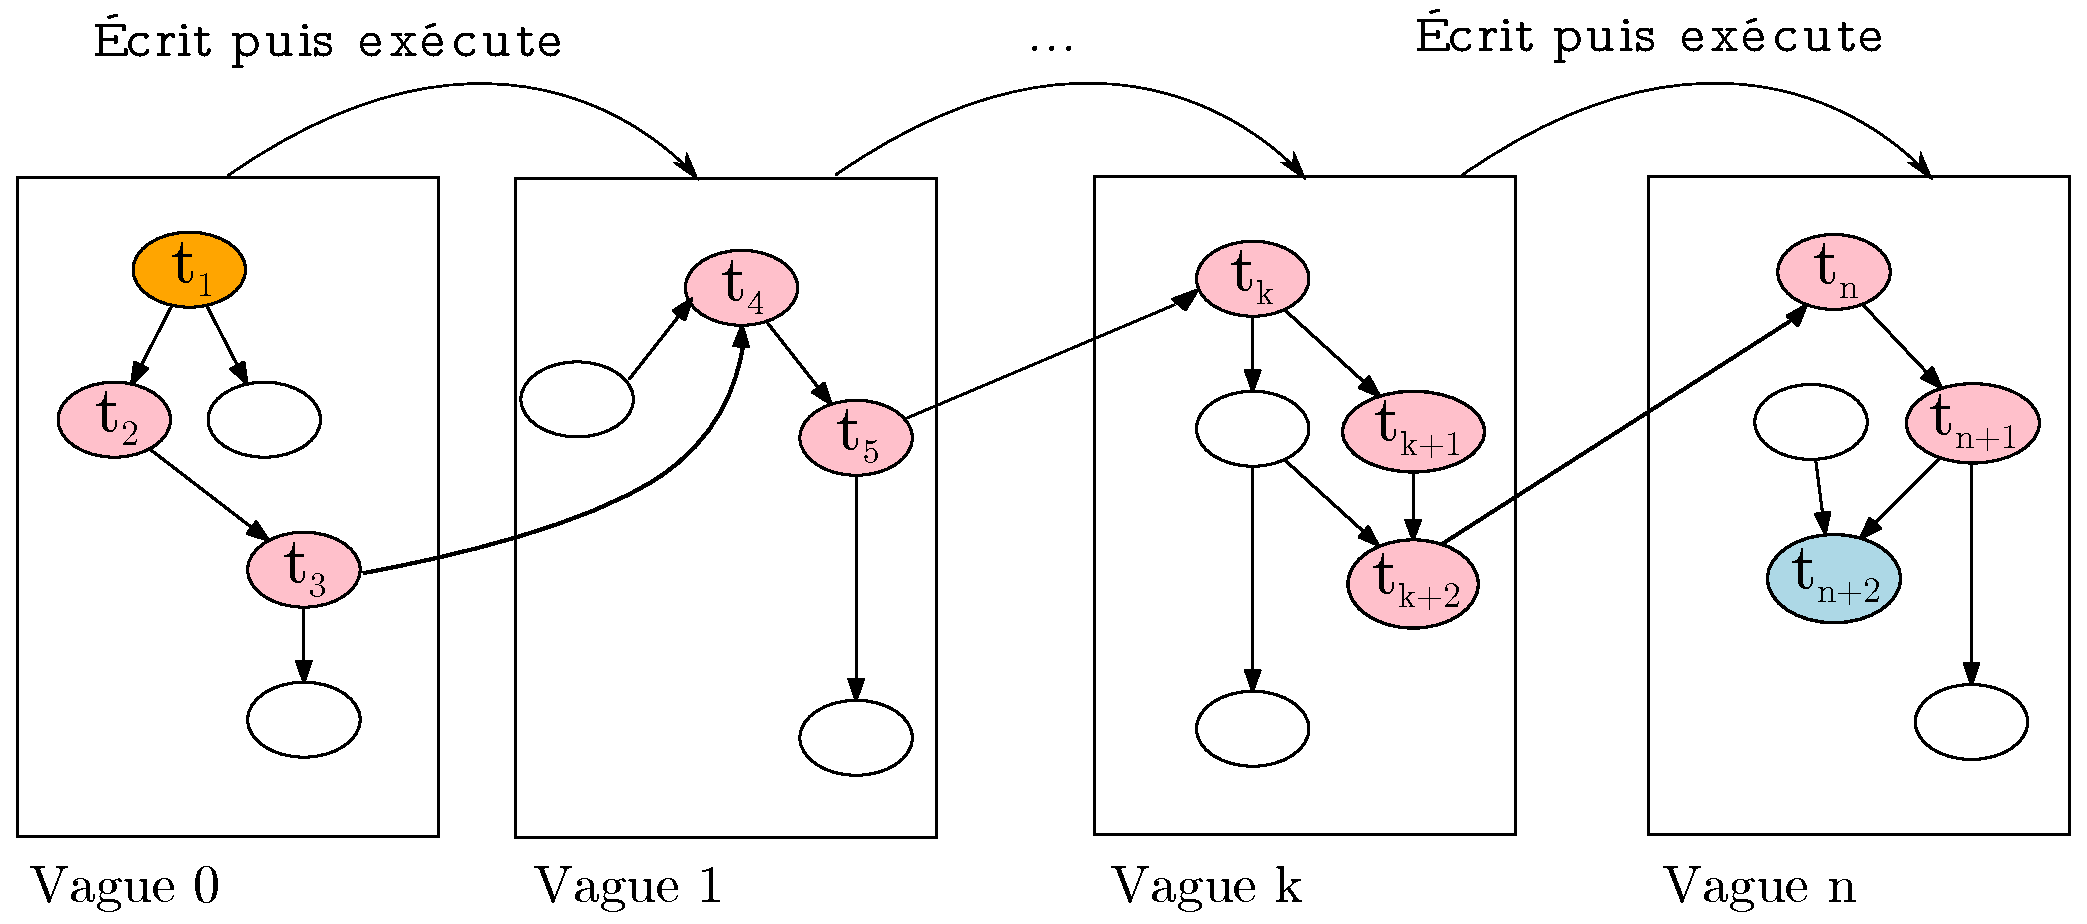
\includegraphics[width=0.8\textwidth]{supports/automodification/phases2_final_test.pdf}
\end{center}

\begin{itemize}
 \item Instantané $i$ : état de la mémoire au début de la vague $i$
 \item Au sein d'une vague, il n'y pas d'auto-modification
\end{itemize}
\end{frame}

\begin{frame}{Auto-modification : graphe de flot de contrôle parfait}
Sans auto-modification :
\begin{itemize}
 \item Donnée : ensemble des traces possibles
 \item Sommet : (adresse, instruction)
 \item Arc : s'il existe une trace dans laquelle les instructions se suivent
\end{itemize}
Avec auto-modification :
\begin{itemize}
 \item Données : ensemble des traces possibles et découpées en niveaux d'exécution
 \item Représenter les niveaux d'exécution dans le GFC ?
\end{itemize}
\end{frame}

\begin{frame}{Auto-modification : exemple}
% \begin{center}
% \subfigure[]{
\begin{tabular}[b]{|l|l|l|l|}
\hline
Adresse & Octets & Instruction & Écriture\\ 
\hline
 8048060 (debut)  &  31 ff             &  xor    edi,edi		& \\
 8048062  &  40                        &  inc    eax			& \\
 8048063  &  74 07                     &  je     804806c (si\_zero) 	& \\
 	  &			       &				& \\
 8048065  &  bf 02 00 00 00            &  mov    edi, 0x2 		& \\
 804806a  &  eb f4                     &  jmp    8048060 (debut) 	& \\
	  &			       &				& \\
 804806c (si\_zero) &  bf 01 00 00 00  &  mov    edi, 0x1 		& \\
 8048071  &  bb 60 80 04 08            &  mov    ebx, 0x8048060 	& \\
 8048076  &  66 c7 03 47 00            &  mov    [ebx], 0x47 		& inc edi\\
 804807b  &  66 c7 43 01 47 00         &  mov    [ebx+0x1], 0x47	& inc edi \\
 8048081  &  66 c7 43 03 c3 00         &  mov    [ebx+0x3], 0xc3	& ret \\
 8048087  &  eb d7                     &  jmp    8048060 (debut) 	& \\
\hline
\end{tabular}
% \end{center}
\vskip-0.5ex
\begin{itemize}
 \item Valeur de \edi\ lorsque \ret\ est atteint ?
\end{itemize}

\end{frame}

\begin{frame}{GFC ne traitant pas l'auto-modification}
\begin{itemize}
 \item Sommet : (adresse, instruction)
\end{itemize}

% \begin{minipage}{0.45\textwidth}
\begin{center}
 \includegraphics[width=0.50\textwidth]{supports/disas_sm/ex2_parfait_cropped0.pdf}
 \end{center}
% \end{minipage}
% \begin{minipage}{0.55\textwidth}
\pause
\begin{itemize}
 \item Certains chemins sont impossibles
 \item On n'observe pas l'enchaînement des niveaux d'exécution
\end{itemize}
% \end{minipage}
\end{frame}

\begin{frame}{Auto-modification : graphe de flot de contrôle paramétré}
\begin{minipage}{0.45\textwidth}
\begin{center}
 \includegraphics[width=1.05\textwidth]{supports/disas_sm/ex2_vagues_cropped0.pdf}
\end{center}
\end{minipage}
\begin{minipage}{0.5\textwidth}
% \begin{itemize}

% \end{itemize}
\begin{itemize}
%  \item Une trace + analyse statique
 \item Sommet : (niveau d'exécution, adresse, instruction)
% \pause
%  \item S'il y a plusieurs traces 
\end{itemize}
\end{minipage}
\end{frame}


% \subsection{Notre approche}
\begin{frame}[t]{Graphe de flot de contrôle parfait}
\only<1>{
\begin{itemize}
 \item On considère toutes les exécutions possibles
 \item Au sein d'une trace, un instantané de la mémoire est associé à chaque niveau d'exécution
\end{itemize}
}
\only<2->{
% \begin{center}
\begin{tabular}{|l|c|c|c|c|c|r}
\cline{1-6}
Niveau d'exécution & 1 & 2 & 3 & 4 & 5 & \\
\cline{1-6}
Trace 1 & $s_1$ & $s_2$ & $s_3$ & $s_4$ & & \\
Trace 2 & $s_1$ & $s_2$ & $s_3$ & $s_5$ & $s_6$ & Instantanés de la mémoire\\
Trace 3 & $s_1$ & $s_2$ & $s_7$ & $s_5$ & $s_6$ & \\
Trace 4 & $s_1$ & $s_2$ & $s_4$ &       & & \\
\cline{1-6}
\end{tabular}
% \end{center}
}

\only<3>{
\begin{center}
\scalebox{0.9}{
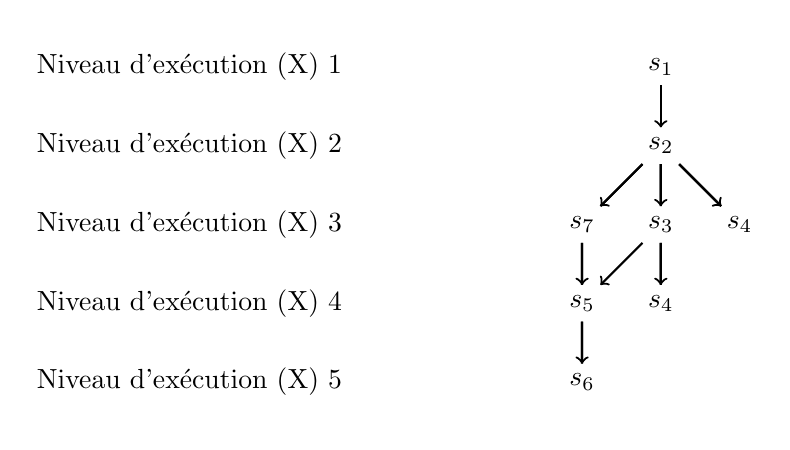
\begin{tikzpicture}[
%   tlabel/.style={pos=0.4,right=-1pt},
%   every node/.style={color=black, circle, minimum size=10mm, draw=black, align=center},
%   edge from parent/.style={->, draw=black},
  level 1/.style={sibling distance=10mm, level distance=10mm},
  thick
]
\node (ROOT) {$s_1$}
% \node (S11){Site 1};
child {node (S2) {$s_2$}
child{node (S3) {$s_7$}
child {node (S4) {$s_5$}
  child {node (S6) {$s_6$}}
}
}
child{node (S7) {$s_3$}
child {node (S8) {$s_4$}
}
}
child {node (S9) {$s_4$}}
};
% \draw (S4) -> (S5);
\path (ROOT) edge [->] (S2);
\path (S2) edge [->] (S3);
\path (S2) edge [->] (S7);
\path (S2) edge [->] (S9);
\path (S3) edge [->] (S4);
\path (S4) edge [->] (S6);
\path (S7) edge [->] (S8);
\path (S7) edge [->] (S4);
\node[draw=none, left=2.5cm of ROOT.west, anchor=east, text width=5cm, minimum size=1cm] (V1){Niveau d'exécution (X) 1};
\node[draw=none, left=2.5cm of S2.west, anchor=east, text width=5cm, minimum size=1cm] (V2){Niveau d'exécution (X) 2};
\node[draw=none, left=2.5cm of S7.west, anchor=east, text width=5cm, minimum size=1cm] (V3){Niveau d'exécution (X) 3};
\node[draw=none, left=2.5cm of S8.west, anchor=east, text width=5cm, minimum size=1cm] (V4){Niveau d'exécution (X) 4};
\node[draw=none, left=1.5cm of S6.west, anchor=east, text width=5cm, minimum size=1cm] (V5){Niveau d'exécution (X) 5};
% \node[draw=none, left=4cm of ROOT.west, anchor=east, text width=1.1cm, minimum size=1.2cm] (V1){Vague 1};
% \node[draw=none, left=4cm of ROOT.west, anchor=east, text width=1.1cm, minimum size=1.2cm] (V1){Vague 1};
% \node[draw=none, left=4cm of ROOT.west, anchor=east, text width=1.1cm, minimum size=1.2cm] (V1){Vague 1};
\end{tikzpicture}
}
\end{center}
}

\only<4>{
\begin{itemize}
 \item Sommet : (niveau d'exécution, instantané, adresse, instruction)
\end{itemize}

% \vskip10ex
\begin{center}
  %TODO : illustration interactive dans plusieurs directions
  \includegraphics[width=1.0\textwidth]{supports/disas_sm/plus_que_parfait_soutenance_cropped0.pdf}
\end{center}
}
\end{frame}

\begin{frame}{Désassemblage hybride}
Analyse dynamique puis statique par parcours récursif
% \begin{itemize}
%  \item Trace séparée en niveaux d'exécution et en instantanés
%  \item Désassemblage statique des instantanés
%  \item Construction du GFC paramétré
% %  \item Construction des couches de code (chevauchement)
% \end{itemize}

\begin{center}
\scalebox{0.8}{
\begin{tikzpicture}[->,scale=1,>=stealth',thick]
\newcommand\espace{0.3cm}
\node[state] (BIN){Binaire};
\node[state, above right=2cm and 3.8cm of BIN] (TRACE) {Trace};
\node[state, below=1.8cm of TRACE.west, anchor=west] (I0) {Instantané 1};
\node[state, below=3.0cm of TRACE.west, anchor=west] (I1) {Instantané 2};
\node[state, below=4.2cm of TRACE.west, anchor=west] (Ip) {Instantané ...};
\node[state, below=5.4cm of TRACE.west, anchor=west] (In) {Instantané n};
% \node[state, right=1.4cm  of BIN] (ASM){ASM};
% \node[state, right=1.4cm of ASM] (IR){LI};

\node[state, right=4cm of I0] (V0) {Vague 1};
\node[state, below=1.2 of V0.west, anchor=west] (V1) {Vague 2};
\node[state, below=2.4 of V0.west, anchor=west] (Vp) {Vague ...};
\node[state, below=3.6 of V0.west, anchor=west] (Vn) {Vague n};

\coordinate [right=2cm of BIN.east] (DYN);
\coordinate [right=1.6cm of TRACE.east] (C0);
\coordinate [right=0.5cm of C0] (C1);
\coordinate [right=0.5cm of C1] (Cp);
\coordinate [right=0.5cm of Cp] (Cn);
% \coordinate [above=0.1cm of C1] (C10m);
% \coordinate [below=0.1cm of C1] (C10p);
\draw [-] (TRACE.east) -- (C0);
\draw [-] (C0) -- (C1);
\draw [-] (C1) -- (Cp);
\draw [-] (Cp) -- (Cn);
\draw (C0) -- ($(C0)+(0, -1.8cm)$);
\draw (C1) -- ($(C1)+(0, -3cm)$);
\draw (Cp) -- ($(Cp)+(0, -4.2cm)$);
\draw (Cn) -- ($(Cn)+(0, -5.4cm)$);
% \draw (C1) -- (C10m);
% \draw (C10p) -- ($(C1)+(0, -1.8cm)$);
\draw [-] (BIN.east) -- node[below left=3.0cm and -3.2cm, text width=4cm](DYNAMIC){Analyse dynamique} (DYN);
\draw (DYN) |- (TRACE.west);
\draw (DYN) |- (I0.west);
\draw (DYN) |- (I1.west);
\draw (DYN) |- (Ip.west);
\draw (DYN) |- (In.west);
\draw (I0) -- (V0);
\draw (I1) -- (V1);
\draw (Ip) -- (Vp);
\draw (In) -- node[below right=0.5cm and -1.8cm, text width=4cm](STATIC){Analyse statique} (Vn);
\node [fit={($(V0.north west) + (-0.2, 0)$) ($(V1) + (0.0, 0)$) ($(Vp) + (0.0, 0)$) ($(Vn.south east) + (0.3, 0)$)}, draw, label=GFC paramétré par la trace] {};
\end{tikzpicture}
}
\end{center}
\end{frame}

\begin{frame}{Exemple sur \hostname\ obscurci}
% \vskip-1ex
\only<1-2>{
\begin{itemize}
 \item Utilisation d'un binaire (\hostname) et de 34 versions obscurcies
%  \item Extraction des graphes de flot de contrôle par analyse hybride
\end{itemize}

\pause
% \vskip-2ex
% Résultats de l'analyse hybride :
\begin{tiny}
\begin{longtable}{|c|c|c|c|c|c|c|c|c|c|c|c|}
\hline
Empaqueteur & Vague & \multicolumn{2}{c|}{Instructions} & \multicolumn{2}{c|}{Instructions en} & \multicolumn{2}{c|}{Couches} & \multicolumn{2}{c|}{Sauts entre}\\
 &  & \multicolumn{2}{c|}{} & \multicolumn{2}{c|}{chevauchement} & \multicolumn{2}{c|}{} & \multicolumn{2}{c|}{couches}\\
  &   & Trace & Désas & Trace & Désas & Trace & Désas & Trace & Désas\\
\hline
\endhead
\rowcolor{lightgray}(aucun) & / & 154 & 354 & / & / & / & / & / & /\\
  & 0 & 154 & 354 & 0 & 0 & 1 & 1 & 0 & 0\\
\hline
\hline
\rowcolor{lightgray}UPX & / & 322 & 523 & / & / & / & / & / & /\\
  & 0 & 168 & 169 & 4 & 4 & 2 & 2 & 2 & 2\\
  & 1 & 154 & 354 & 0 & 0 & 1 & 1 & 0 & 0\\
\hline
\rowcolor{lightgray}tElock99 & / & 2044 & 3022 & / & / & / & / & / & /\\
  & 0 & 46 & 130 & 0 & 42 & 1 & 3 & 0 & 16\\
  & \multicolumn{9}{c|}{...}\\
  & 2 & 19 & 20 & 2 & 2 & 2 & 2 & 2 & 2\\
  & 3 & 25 & 25 & 8 & 8 & 2 & 2 & 8 & 8\\
  & \multicolumn{9}{c|}{...}\\
  & 17 & 226 & 430 & 0 & 0 & 1 & 1 & 0 & 0\\
\hline
\end{longtable}
\end{tiny}

% \pause
% \vskip-3ex
\begin{itemize}
 \item 28/34 binaires ont atteint la charge finale (\hostname)
 \item 27/28 sont auto-modifiants : de 2 à 79 vagues
\end{itemize}
}

\only<3>{
\begin{itemize}
 \item 22/28 ont plusieurs couches de code dans le désassemblage
 \begin{itemize}
  \item de 2 à 4 couches
  \item de nombreux sauts entre couches (jusqu'à 1 817 pour jdpack)
 \end{itemize}
\vskip4ex
 \item 9/28 (\telock, \upx, pespin) exécutent réellement des instructions en chevauchement
 \begin{itemize}
  \item uniquement 2 couches
  \item jusqu'à 12 sauts entre couches
 \end{itemize}
\end{itemize}}
\end{frame}

% \begin{frame}{CFG de la vague 2 de \telock}
%  \begin{center}
%   \includegraphics[width=0.33\textwidth]{supports/disas_sm/telock_v2_cropped0.pdf}
% \end{center}
% \end{frame}


% \begin{frame}{Rappels}
% \begin{itemize}
%  \item Désassemblage et analyse de codes protégés
%  \item Traitement du chevauchement de code (analyse statique)
%  \item Traitement de l'auto-modification (analyse dynamique)
%  \item Combinaison des deux afin de reconstruire un graphe de flot de contrôle cohérent
% \end{itemize}
% \end{frame}

\section{Algorithmes de comparaison}
\titre{Analyse morphologique et algorithmes de comparaison de graphes}

\begin{frame}{Analyse morphologique}
% Analyse morphologique :
\begin{itemize}
 \item Comparaison des graphes de flot de contrôle
 \item Détection par signatures
\end{itemize}

\begin{center}
\scalebox{0.8}{
\begin{tikzpicture}[->,scale=1,>=stealth',thick]
\newcommand\espace{0.3cm}
\node[state] (BIN){Binaire};
\node[state, right=3.8cm of BIN.west, anchor=west] (CODE) {Code};
\node[state, above=1.2cm of CODE.west, anchor=west] (TRACE) {Traces};
\node[state, below=1.2cm of CODE.west, anchor=west] (GFC) {GFC};
\coordinate [right=1cm of BIN.east] (DYN);
\coordinate [right=4cm of DYN] (CLASS);
\coordinate [right=1cm of CLASS] (IN);
\coordinate [right=1cm of IN] (OUT);
% \node[state, above=2cm of IN] (COMP) {Liste de comportements};
\node[state, above=2cm of IN] (SIG) {Corpus de programmes classés};
\node[state, above right=1cm and 1cm of OUT, anchor=west] (MAL) {Malveillant};
\node[state, below right=1cm and 1cm of OUT, anchor=west] (LEG) {Légitime};
\draw [-] (BIN.east) -- node[below left=1.6cm and -3.2cm, text width=4cm](DYNAMIC){Extraction} (DYN);
\draw [-] (CLASS) -- (IN);
\draw [-] (IN) -- node[below right=1.6cm and -1.8cm, text width=4cm](STATIC){Classification} (OUT);
\draw (DYN) |- (TRACE.west);
\draw (DYN) |- (CODE.west);
\draw (DYN) |- (GFC.west);
\draw (OUT) -- (MAL.west);
\draw (OUT) -- (LEG.west);
% \draw (COMP.south) -- (IN);
\draw (SIG.south) -- (IN);
\draw [-] (TRACE.east) -| (CLASS);
\draw [-] (CODE.east) -| (CLASS);
\draw [-] (GFC.east) -| (CLASS);
% \draw (In) --  (Vn);
% \node [fit={($(V0.north west) + (-0.2, 0)$) ($(V1) + (0.0, 0)$) ($(Vp) + (0.0, 0)$) ($(Vn.south east) + (0.3, 0)$)}, draw, label=GFC paramétré par la trace] {};
\end{tikzpicture}
}
\end{center}

\begin{itemize}
 \item Les signatures sont des graphes de flot de contrôle
 \item On cherche des isomorphismes de sous-graphes
\end{itemize}

\end{frame}



% \begin{frame}{Analyse morphologique et similarité logicielle\footnote{Bonfante, Calvet, Marion, Sabatier, Thierry (REcon 2012, Malware 2012)}}
% Problème : Waledac et OpenSSL
%  
% \begin{itemize}
%   \item Analyser un binaire : Waledac
%   \item Pas d'informations de compilation (nom des fonctions)
%   \item Utilise OpenSSL
% \end{itemize}
% 
% \pause
% Objectif :
% \begin{itemize}
%   \item Correspondance fine entre instructions
%   \item Identification automatique des fonctions
% \end{itemize}
% 
% \pause
% Analyse morphologique :
% \begin{itemize}
% \item Comparaison des graphes de flot de contrôle
% \item Recherche d'isomorphismes de sous-graphes
% \item Détection de logiciels malveillants (par signature)
% \end{itemize}
% Comment formaliser et optimiser cette approche ?
% \end{frame}

% \begin{frame}{Détection et analyse morphologique}
% %  Analyse morphologique
%  \begin{itemize}
%   \item Approche de détection par signatures
%  \end{itemize}
% \begin{center}
% 
% \scalebox{0.9}{
% \begin{tikzpicture}[->,scale=1,>=stealth',thick]
% \newcommand\espace{0.3cm}
% \node[state] (BIN){Binaire};
% \node[state, right=3.8cm of BIN.west, anchor=west] (CODE) {Code};
% \node[state, above=1.2cm of CODE.west, anchor=west] (TRACE) {Traces};
% \node[state, below=1.2cm of CODE.west, anchor=west] (GFC) {GFC};
% \coordinate [right=1cm of BIN.east] (DYN);
% \coordinate [right=4cm of DYN] (CLASS);
% \coordinate [right=1cm of CLASS] (IN);
% \coordinate [right=1cm of IN] (OUT);
% % \node[state, above=2cm of IN] (COMP) {Liste de comportements};
% \node[state, above=2cm of IN] (SIG) {Corpus de programmes classés};
% \node[state, above right=1cm and 1cm of OUT, anchor=west] (MAL) {Malveillant};
% \node[state, below right=1cm and 1cm of OUT, anchor=west] (LEG) {Légitime};
% \draw [-] (BIN.east) -- node[below left=1.6cm and -3.2cm, text width=4cm](DYNAMIC){Extraction} (DYN);
% \draw [-] (CLASS) -- (IN);
% \draw [-] (IN) -- node[below right=1.6cm and -1.8cm, text width=4cm](STATIC){Classification} (OUT);
% \draw (DYN) |- (TRACE.west);
% \draw (DYN) |- (CODE.west);
% \draw (DYN) |- (GFC.west);
% \draw (OUT) -- (MAL.west);
% \draw (OUT) -- (LEG.west);
% % \draw (COMP.south) -- (IN);
% \draw (SIG.south) -- (IN);
% \draw [-] (TRACE.east) -| (CLASS);
% \draw [-] (CODE.east) -| (CLASS);
% \draw [-] (GFC.east) -| (CLASS);
% % \draw (In) --  (Vn);
% % \node [fit={($(V0.north west) + (-0.2, 0)$) ($(V1) + (0.0, 0)$) ($(Vp) + (0.0, 0)$) ($(Vn.south east) + (0.3, 0)$)}, draw, label=GFC paramétré par la trace] {};
% \end{tikzpicture}
% }
% \end{center}
% 
% \begin{itemize}
% \item Les signatures sont des graphes de flot de contrôle
% \item On cherche des isomorphismes de sous-graphes
% \end{itemize}
% \end{frame}

\begin{frame}[t]{Isomorphisme appliqué aux graphes de flot}
% \begin{itemize}
%  \item 
 Les graphes sont réduits :
 \begin{itemize}
  \item But : rendre les signatures plus génériques
  \item Instructions : \texttt{call eax} $\rightarrow$ \texttt{CALL}
  \item Regroupement des instructions séquentielles : bloc $\rightarrow$ \texttt{INST}
 \end{itemize}
% \end{itemize}

\pause
\vskip3ex
Isomorphisme de sous-graphes :
\begin{itemize}
 \item Appliqué entre des graphes de flot extraits d'un malware (signatures) et le graphe à analyser
 \item Problème NP complet
 \item Algorithme classique (Ullmann\only<2>{\footnote{J.R. Ullmann, ``An algorithm for Subgraph Isomorphism'' (1976)}}) trop lent
\end{itemize}
\vskip3ex
Objectif : définir un sous-problème $\rightarrow$ solutions en temps polynomial ?
\end{frame}

\begin{frame}{Simplification : graphes de flot et sites}
% \only<1->{
Graphe de flot :
\begin{itemize}
 \item Le nombre de fils est borné (par 2)
 \item Les fils sont ordonnés
\end{itemize}
On génère des sous-graphes (sites) par parcours en largeur de taille fixe
\begin{itemize}
 \item Site : graphe de flot avec racine
\end{itemize}

% }

% \only<2-3>{
% \begin{block}{Définition : Graphe de flot}
% Un graphe de flot est un graphe orienté et étiqueté vérifiant :
% \begin{enumerate}
% %  \item Chaque sommet a une étiquette, et
% %  \begin{enumerate}
% %   \item La valence d'un sommet est son nombre de fils
% \item Il y a une borne $k$ sur le nombre de fils des sommets% (2 dans le cas d'un \texttt{jcc})
%  \item Les fils de chaque sommet sont ordonnés :
% %  les arcs ont pour label l'ordre i du fils (où i est un entier compris entre 1 et la valence du sommet)\\
% %        l'ensemble des arcs est $E\subset V\times \mathbb{N}\times V$. 
%        le numéro $i$ d'un fils du sommet $s$ vérifie
%        \begin{itemize}
%         \item $1\leq i\leq k$, et
% %         \item il y a un arc numeroté i entre le sommet t et le sommet h, et
%         \item $s$ n'a pas d'autre fils numéroté i.% : $\{(t, i, h')\in E, h'\ne h\}=\emptyset$.
%        \end{itemize}
% %  \item La valence de ses sommets est bornée
% \end{enumerate}
% \end{block}
% }
% 
% \only<3>{
% \begin{block}{Définition : Site}\label{def-site}
% Un site P est un graphe de flot ayant une racine : il existe un sommet à partir duquel on peut atteindre n'importe quel autre sommet de P.
% \end{block}
% }

% \only<2>{
% \begin{center}
% \def\imagetop#1{\vtop{\null\hbox{#1}}}
% \pause
\vskip1ex
\begin{tabular}{|c|c|}
\hline
Graphe de flot & Signature : ensemble de sites\\
% \hline
\includegraphics[width=0.25\textwidth]{supports/algos/g1gf_cropped0.pdf}
&
\includegraphics[width=0.6\textwidth]{supports/algos/g1_sites_cropped0.pdf}
% &
% \imagetop{\includegraphics[width=0.2\textwidth]{supports/algos/g1_prof_cropped10.pdf}}
\\
\hline
\end{tabular}
% \pause
% \vskip1ex
% Isomorphisme entre un site et un sous-site d'un graphe de flot ?
% \end{center}
% }
\end{frame}


\begin{frame}[t]{Parcours d'un site}
% \begin{center}
\begin{tabular}{|c|c|c|}
\hline
Site & Numérotation  & Numérotation\\
 & en profondeur & en largeur\\
\hline
\includegraphics[width=0.25\textwidth]{supports/algos/g1_cropped0.pdf}
&
\includegraphics[height=0.37\textwidth]{supports/algos/g1_prof_cropped0.pdf}
&
\includegraphics[height=0.37\textwidth]{supports/algos/g1_larg_cropped0.pdf}
\\
\hline
\end{tabular}
% \end{center}

\only<2>{
\vskip1ex
Codage de parcours en profondeur :\\
$1: JCC\xrightarrow{1} 2: CALL \xrightarrow{1} 3: INST \xrightarrow{1} 4: RET \xrightarrow{R} 2 \xrightarrow{2} 5: RET \xrightarrow{R} 1 \xrightarrow{2} 6:~JCC \xrightarrow{2}~7:INST \xrightarrow{1} 2$.
}

\only<3>{
\vskip1ex
Codage de parcours en largeur :\\
$1: JCC\xrightarrow{1} 2: CALL\xrightarrow{R} 1\xrightarrow{2} 3: JCC\xrightarrow{R} 2\xrightarrow{1} 4: INST\xrightarrow{R} 2\xrightarrow{2} 5: RET \xrightarrow{R} 3 \xrightarrow{2}~6:~INST \xrightarrow{R} 4\xrightarrow{1} 7: RET$.
}
\end{frame}

\begin{frame}{Codage de parcours}
Codage de parcours en largeur :\\
$1: JCC\xrightarrow{1} 2: CALL\xrightarrow{R} 1\xrightarrow{2} 3: JCC\xrightarrow{R} 2\xrightarrow{1} 4: INST\xrightarrow{R} 2\xrightarrow{2} 5: RET \xrightarrow{R} 3 \xrightarrow{2}~6:~INST \xrightarrow{R} 4\xrightarrow{1} 7: RET$.

\begin{block}{Définition : Mot de parcours}
 Un mot de parcours est soit :
 \begin{itemize}
  \item de type $m_1$, c'est à dire $1:L$ où L est une étiquette, ou
  \item de type $m_2$, c'est à dire $\xrightarrow{\alpha}i[:L]$ où i est un entier, L est une étiquette et $\alpha$ est soit un entier k, soit R.
 \end{itemize}
 \label{def-mot-bien-forme}
\end{block}
Un codage de parcours est de la forme $m_1(m_2)^*$
\end{frame}

\begin{frame}{Codage de parcours}
% Codage de parcours en largeur :\\
% $1: JCC\xrightarrow{1} 2: CALL\xrightarrow{R} 1\xrightarrow{2} 3: JCC\xrightarrow{R} 2\xrightarrow{1} 4: INST\xrightarrow{R} 2\xrightarrow{2} 5: RET \xrightarrow{R} 3 \xrightarrow{2}~6:~INST \xrightarrow{R} 4\xrightarrow{1} 7: RET$.

\begin{block}{Définition : Codage de parcours bien formé}
 Un codage de parcours est dit bien formé s'il vérifie :
\begin{enumerate}
 \item L'étiquette de chaque sommet $i$ est spécifiée une unique fois, lors la première référence à ce sommet
 \item Pour tout mot de la forme $\xrightarrow{R}i$, un mot $i:L$ est présent précédemment dans le codage
 \item Chaque fils de chaque sommet est défini au plus une fois
\end{enumerate} 
\label{def-codage-bien-forme}
\end{block}

\begin{itemize}
 \item Les algorithmes fournissant les parcours en profondeur et en largeur sont simples
 \item Ils produisent des codages de parcours bien formés
 \item On peut reconstruire le site d'origine à partir du codage de parcours bien formé
\end{itemize}
\end{frame}

\begin{frame}{Parcours d'un codage au sein d'un graphe de flot}
Le parcours d'un codage bien formé est-il possible dans un graphe de flot ?

\begin{minipage}{0.5\textwidth}
$1: JCC\xrightarrow{1} 2: CALL\xrightarrow{R} 1\xrightarrow{2} 3: JCC$%\\
% $1: CALL\xrightarrow{1} 2: INST\xrightarrow{R} 1\xrightarrow{2} 3: RET$
\end{minipage}
\begin{minipage}{0.4\textwidth}
\begin{center}
\includegraphics[width=0.7\textwidth]{supports/algos/g1p_cropped0.pdf}
\end{center}
\end{minipage}

\pause
\begin{itemize}
\item On part de chaque sommet du graphe à analyser
\item On cherche à réaliser le parcours à partir de ce sommet
\item Le codage est traité mot après mot
\end{itemize}

% \pause
% Exemple supplémentaire :\\
% $1: CALL\xrightarrow{1} 2: INST\xrightarrow{R} 1\xrightarrow{2} 3: RET$
\end{frame}

\begin{frame}{Codages et isomorphisme de sous-graphes}
% \only<1->{
Lien entre isomorphisme de sous-graphes et parcours dans un graphe de flot ?
% }

\pause
% \only<2->{
\begin{theo}
 Soit P un site et T un graphe de flot. Les propositions suivantes sont équivalentes.
 \begin{itemize}
  \item P est isomorphe à un sous-site de T.
  \item Tout codage de parcours bien formé de P peut être parcouru dans T.
  \item Il existe un codage de parcours bien formé de P qui peut être parcouru dans T.
 \end{itemize}
\end{theo}
% }

\pause
Conséquence : équivalence entre
\begin{itemize}
 \item P est isomorphe à un sous-site de T
 \item Le codage de parcours en profondeur de P peut être parcouru dans T
 \item Le codage de parcours en largeur de P peut être parcouru dans T
\end{itemize}

% \only<3->{
% \begin{cor}
%  Soit P un site et T un graphe de flot. Les trois propositions suivantes sont équivalentes.
%  \begin{itemize}
%   \item P est isomorphe à un sous-site de T.
%   \item Le codage de parcours en profondeur de P peut être parcouru dans T.
%   \item Le codage de parcours en largeur de P peut être parcouru dans T.
%  \end{itemize}
% \label{cor:gf}
% \end{cor}
% }
\end{frame}

\begin{frame}[t]{Détection d'isomorphismes par parcours de codage}
% \begin{center}
% \def\imagetop#1{\vtop{\null\hbox{#1}}}
\begin{tabular}{|c|c|}
\hline
Sites de la base & Graphe de flot à analyser\\
\includegraphics[width=0.6\textwidth]{supports/algos/g1_sites_cropped5.pdf}
&
\includegraphics[width=0.25\textwidth]{supports/algos/g1p_cropped5.pdf}
% &
% \imagetop{\includegraphics[width=0.2\textwidth]{supports/algos/g1_prof_cropped10.pdf}}
\\
\hline
\end{tabular}
% \end{center}

\pause
\only<2>{
\vskip1ex
Parcours en profondeur :
\begin{itemize}
\item $1: JCC\xrightarrow{1} 2: CALL\xrightarrow{R} 1\xrightarrow{2} 3: JCC$
\item $1: CALL\xrightarrow{1} 2: INST\xrightarrow{R} 1\xrightarrow{2} 3: RET$
\item $1: JCC\xrightarrow{2} 2: INST \xrightarrow{1} 3: CALL$
\item $1: INST\xrightarrow{1} 2: CALL \xrightarrow{1} 3: INST$
\end{itemize}
}
\only<3->{
$1: JCC\xrightarrow{1} 2: CALL\xrightarrow{R} 1\xrightarrow{2} 3: JCC$
\begin{itemize}
\item La possibilité du parcours d'un codage indique s'il y a un isomorphisme
\item Chaque site est testé indépendamment des autres
% \item La complexité temporelle est polynomiale
\end{itemize}
}
% \only<4>{
% $1: CALL\xrightarrow{1} 2: INST\xrightarrow{R} 1\xrightarrow{2} 3: RET$
% }
\end{frame}


\begin{frame}{Détection d'isomorphismes par parcours de codage}
% \begin{minipage}{.40\textwidth}
 \begin{center}
 \scalebox{0.6}{
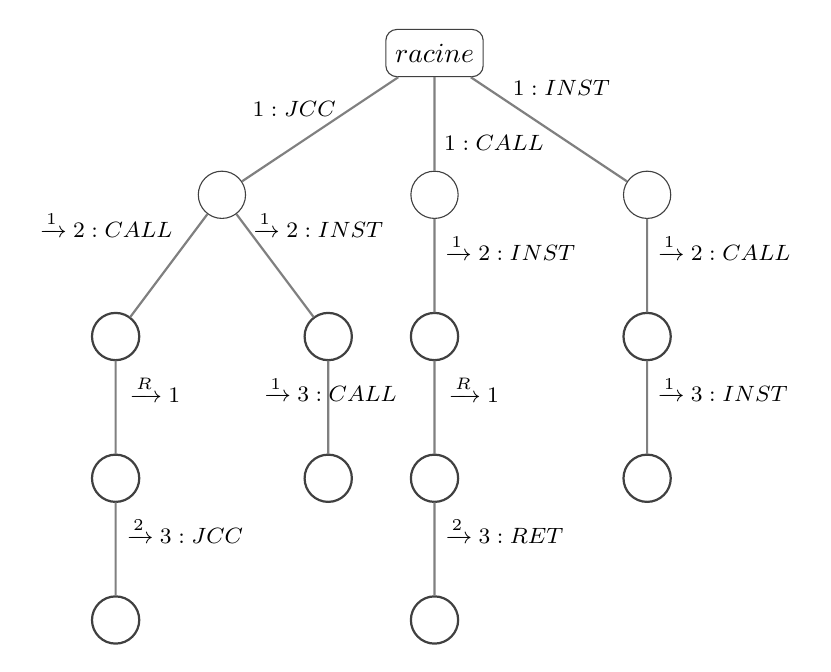
\begin{tikzpicture}[
  tlabel/.style={pos=0.4,right=-1pt,font=\footnotesize\color{black!70!black} },
  every node/.style={color=black!25!black, circle, minimum size=6mm, draw=black!75, align=center},
  edge from parent/.style={draw=black!50,thick},
  level 1/.style={sibling distance=27mm, level distance=18mm},
]
\node[rectangle, rounded corners]{$racine$}
child {node {}
       child{node {}
	     child {node {}
	            child {node {}
		           edge from parent node[tlabel,pos=0.3,draw=none] {$\xrightarrow{2} 3: JCC$}
	            }
	            edge from parent node[tlabel,pos=0.3,draw=none] {$\xrightarrow{R} 1$}
	     }
	     edge from parent node[tlabel,pos=0.1, left=5pt,draw=none] {$\xrightarrow{1} 2: CALL$}
       }
       child{node {}
	     child {node {}
	            edge from parent node[tlabel,pos=0.3, right=-28pt, draw=none] {$\xrightarrow{1} 3: CALL$}
	     }
	     edge from parent node[tlabel,pos=0.1, right=-10pt,draw=none] {$~~~\xrightarrow{1} 2: INST$}
       }
       edge from parent node[tlabel,pos=0.3, left, draw=none] {$1: JCC$}
}
child {node {}
       child{node {}
	     child {node {}
	            child {node {}
		           edge from parent node[tlabel,pos=0.3,draw=none] {$\xrightarrow{2} 3: RET$}
	            }
	            edge from parent node[tlabel,pos=0.3,draw=none] {$\xrightarrow{R} 1$}
	     }
	     edge from parent node[tlabel,pos=0.3,draw=none] {$\xrightarrow{1} 2: INST$}
       }
       edge from parent node[tlabel,pos=0.7,draw=none] {$1: CALL$}
}
child {node {}
       child{node {}
	     child {node {}
	            edge from parent node[tlabel,pos=0.3,draw=none] {$\xrightarrow{1} 3: INST$}
	     }
	     edge from parent node[tlabel,pos=0.3,draw=none] {$\xrightarrow{1} 2: CALL$}
       }
       edge from parent node[tlabel,pos=0.1, right=5pt, draw=none] {$1: INST$}
};
\end{tikzpicture}
}
\end{center}
% \end{minipage}
% \begin{minipage}{.7\textwidth}
Codages rangés dans un arbre :
 \begin{itemize}
  \item Certains parcours sont factorisés
  \item On doit parcourir tous les sommets de l'arbre
%   \item Dépend (au pire) linéairement du nombre de sites dans la base
 \end{itemize}
% \end{minipage}
\end{frame}


\begin{frame}{Approche par découpage}
Autre approche :
 \begin{itemize}
  \item Découper également le graphe de flot du programme à analyser en sites
  \item Recherche d'isomorphismes de sites
 \end{itemize}
 
\pause
Dans ce cas :
\begin{itemize}
 \item Un site a une représentation unique (matricielle)
 \item On peut ranger les sites dans un arbre de hauteur fixe
 \item La détection d'un site revient à la recherche dans un arbre ordonné
\end{itemize}

\pause
Conséquences :
\begin{itemize}
 \item La complexité ne dépend plus du nombre de sites dans la base
 \item Mais l'algorithme n'est pas complet
\end{itemize}
\end{frame}


\begin{frame}{Complexité en temps dans le pire des cas}
Problème :
\begin{itemize}
 \item Isomorphisme de sous-graphes
 \item Dans le cas des graphe de flot et des sites
\end{itemize}

\vskip2ex
\begin{itemize}
 \item n : taille du graphe de flot
 \item S : nombre de sites dans la base
 \item W : taille des sites considérés (en pratique 24)
\end{itemize}

\begin{center}
\begin{tabular}{|c|c|c|c|}
 \hline
 Algorithme & Ajout d'un & Analyse d'un & Complet\\
   & graphe de flot & graphe de flot & \\
 \hline
 Recherche exhaustive & / & $O(S.n^3.n!)$ & Oui\\
 Ullmann & / & $O(S.(n/3)^W)$ & Oui \\
 Parcours & $O(n.W^2)$ & $O(S.n.W)$ & Oui\\
 Découpage & $O(n.W^3)$ & $O(n.W^2)$ & Non\\
 \hline
\end{tabular} 
\end{center}
\end{frame}

\begin{frame}[t]{Implémentations : performance}
\begin{itemize}
% 17044
% 4 452 219
 \item Base de programmes malveillants : 465 000 sites uniques
%  \only<2->{
 \item Apprentissage : croissance linéaire, $<$ 6 minutes
%  }
 \pause
 \item Détection de 5 programmes (18 160 sites) en fonction du nombre de sites appris
\end{itemize}

% \begin{figure}[h]

Parcours :
\begin{center}
% 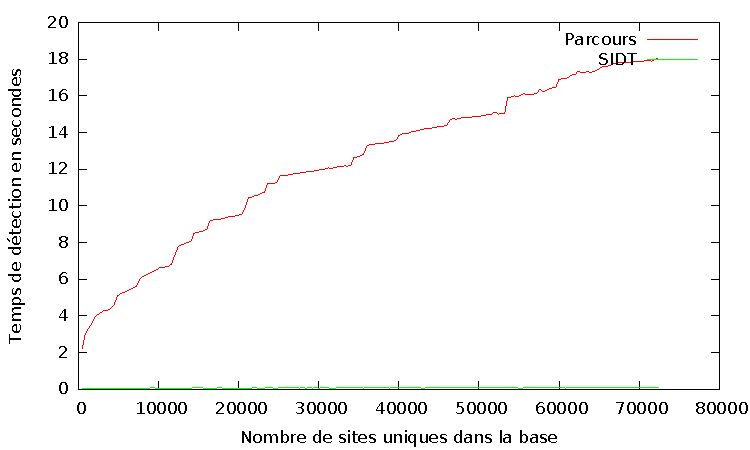
\includegraphics[width=0.9\textwidth]{supports/plots/plotScan.pdf}
% \only<2>{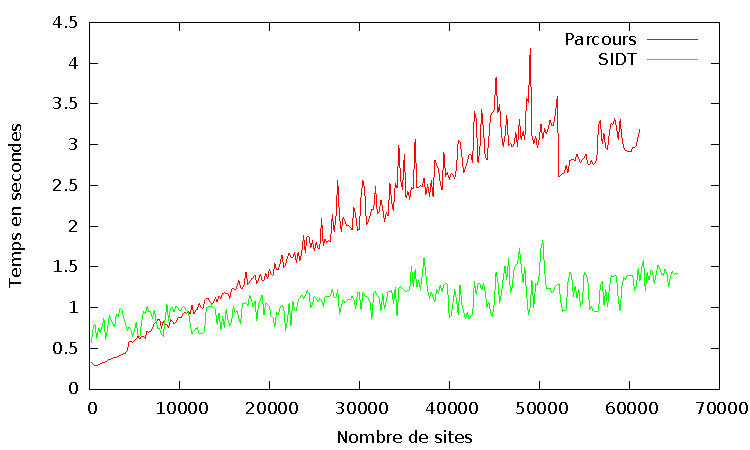
\includegraphics[width=0.65\textwidth]{supports/plots/plotLearn.pdf}}
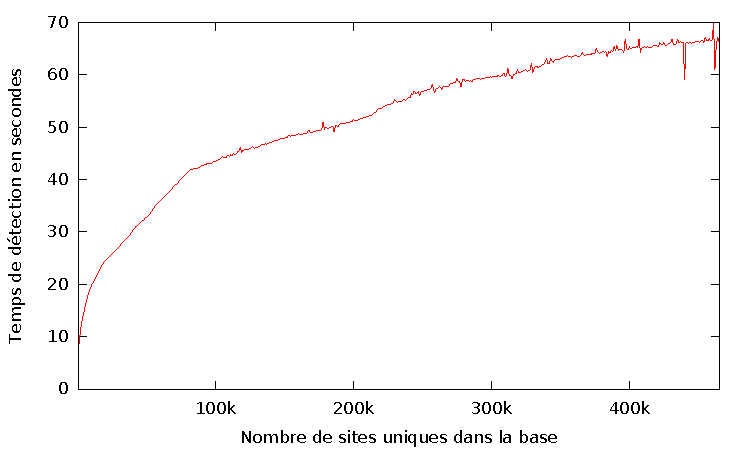
\includegraphics[width=0.65\textwidth]{supports/plots/plotScan-plus-GTSI.pdf}
\end{center}
\vskip-1.5ex Découpage : $<$ 1 seconde
% \caption{}
% \label{fig:scan}
% \end{figure}
\end{frame}

\begin{frame}{Retour sur \hostname\ protégé}
\vskip-3ex
\begin{itemize}
 \item Utilisation d'un binaire (\hostname) et de 34 versions protégées
 \item Extraction des graphes de flot de contrôle par analyse hybride
 \item Comparaison des graphes de flot par analyse morphologique
\end{itemize}

\pause
\vskip1ex
Résultats :
\begin{itemize}
 \item 28/34 binaires ont pu être analysés dynamiquement
 \item Dans 24/28 cas, on détecte plus de 75\% des sites de \hostname\ dans la version protégée
\end{itemize}

\pause
\vskip1ex
Comparaison des algorithmes de détection :
\vskip1ex
% \begin{center}
\begin{tabular}{|c|c|c|c|c|}
\hline
 Algorithme & Apprentissage & Détection & Sites uniques & Détection\\
   &  &  & détectés & à + de 75\%\\
 \hline
%  Ullmann & $\infty$ & $\infty$ & (6739) & (24)\\
 Parcours & $<$ 1 seconde & 70 secondes & 6 739 & 24/28\\
 Découpage & $<$ 1 seconde & 1.6 seconde & 6 045 & 22/28\\
 \hline
\end{tabular}
% \end{center}
\end{frame}

\section{Similarité logicielle}
\titre{Détection de similarités logicielles}

\begin{frame}[t]{Similarité logicielle}
Problème : comparaison de deux programmes\\
\vskip1ex
Objectif : détecter de parties de code en commun

\pause
\vskip2ex
Analyse morphologique :
\begin{itemize}
  \item Découpage entre sites
  \item Correspondance entre sites
\end{itemize}

\pause
\vskip2ex
Adaptation :
\begin{itemize}
  \item Correspondance fine entre instructions
  \item Identification automatique de fonctions
\end{itemize}

\vskip2ex
Implémentation :
\begin{itemize}
 \item Avec l'algorithme par découpages
 \item Plugin pour IDA : affiche les similarités détectées
\end{itemize}


\end{frame}


\begin{frame}[t]{Waledac et OpenSSL\only<3>{\footnote{Bonfante, Calvet, Marion, Sabatier, Thierry (REcon 2012, Malware 2012)}}}
\only<1,3>{
 Problème :
\begin{itemize}
  \item Analyser un programme malveillant : Waledac
  \item Pas d'informations de compilation (nom des fonctions)
  \item Utilise OpenSSL : Quelles fonctions sont utilisées ?
\end{itemize}
}

\only<2>{
\vskip-2ex
\begin{itemize}
 \item Analyse morphologique et alignement du code
\end{itemize}
\vskip1ex
\begin{center}
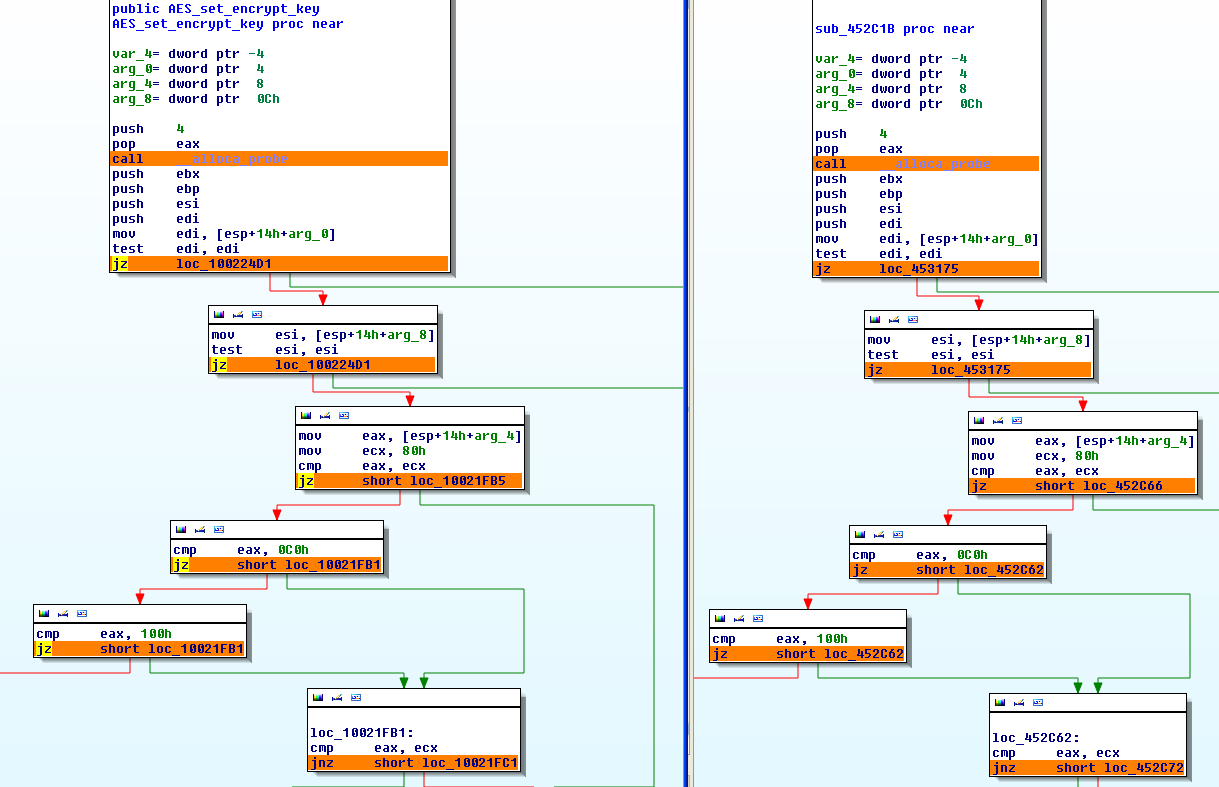
\includegraphics[width=0.8\textwidth]{supports/libs/WalSSLIDAAESgraph.png}
\end{center}
\begin{itemize}
 \item IDA : OpenSSL à gauche, Waledac à droite
\end{itemize}

}

\only<3>{
\vskip3ex
\begin{tabular}{|p{7cm}|l|}
\hline
Fonctions                                      & Fonctionnalité                        \\
\hline
AES\_set\_encrypt\_key, AES\_set\_decrypt\_key         & Chiffrement AES                       \\
RSA\_free, DSA\_size, DSA\_new\_method                 & Chiffrement RSA / DSA                 \\
X509\_PUBKEY\_set, X509\_PUBKEY\_get 				& Certificats X509 			\\
BN\_is\_prime\_fasttest\_ex, BN\_ctx\_new	& Gestion des grands entiers	\\
CRYPTO\_lock, CRYPTO\_malloc                   & Fonctions génériques  \\
\hline
\end{tabular}
}
\end{frame}


\begin{frame}[t]{Similarité logicielle : Duqu et Stuxnet\footnote{Bonfante, Marion, Sabatier, Thierry (SSTIC 2013, Malware 2013)}}
Application à Duqu (2011) et Stuxnet (2010)
\begin{itemize}
%  \item Code en commun ?
 \pause
 \item 26.5\% des sites de \duqu\ en commun avec \stux
 \item 60.3\% des sommets du graphe de flot de \duqu\ correspondent à des sommets de \stux
\end{itemize}

\pause
\vskip2ex
La charge finale de \duqu\ est similaire à \stux 
\begin{itemize}
 \item Présente uniquement en mémoire
 \item Comment la détecter avant l'infection ?
 \item \duqu\ surveille les processus pour s'y injecter
\end{itemize}

\pause
\vskip2ex
Rétroingénierie du pilote de \duqu\
\begin{itemize}
 \item Construction d'une version défensive
 \item Capable de détecter une infection par Duqu
\end{itemize}
\end{frame}


\section{}
\titre{Conclusion}

\begin{frame}{Conclusion}
Désassemblage :
\begin{itemize}
\item Analyse et désassemblage de programmes binaires obscurcis
\item Traitement du chevauchement de code
\item Graphe de flot de contrôle pour programmes auto-modifiants
\item Implémentation d'un désassembleur hybride
\end{itemize}

Détection :
\begin{itemize}
\item Comparaison des graphes de flot de contrôle
\item Formalisation et optimisation de l'analyse morphologique
\item Application à la détection de similarités logicielles
\end{itemize}
\end{frame}

\begin{frame}{Perspectives}
Désassemblage :
\begin{itemize}
 \item Évaluer les faux positifs sur un grand nombre d'échantillons
 \item Utiliser des techniques d’interprétation abstraite
 \item Incorporer plusieurs traces dans le même graphe de flot de contrôle
\end{itemize}

Analyse morphologique :
\begin{itemize}
 \item Utiliser d'autres critères du graphe de flot (chevauchements)
 \item Développer des méthodes de réductions résistantes à certains obscurcissements
 \item Étudier en détail la précision (faux positifs, faux négatifs) et l'influence des constantes (taille des sites, seuil de détection)
\end{itemize}
\end{frame}

\begin{frame}%[plain]
\begin{center}	
  \Huge Merci !
\end{center}
\end{frame}


\makeatletter
  \immediate\write\@mainaux{\string\gdef\string\inserttotalframenumbernew{\insertframenumber}}
\makeatother
\appendix


% \begin{frame}[allowframebreaks]
% \section*{}
% {
% \frametitle{Références}
% \bibliography{../rapportbib}
% \bibliographystyle{alpha}
% }
% \end{frame}

% % suppléments :
% \begin{frame}{More}
% \end{frame}




\end{document}
